\documentclass[a4paper,10pt]{article}
\usepackage[utf8]{inputenc}

\usepackage[american]{babel}
\usepackage{graphicx}
\usepackage{amsmath}
\usepackage{amsthm}
\usepackage{amssymb}
\usepackage{natbib}
\usepackage[margin=0.5in]{geometry}
\usepackage{fancyvrb}
\usepackage{pdfpages}
\usepackage{xcolor,colortbl}

\setlength{\parskip}{.1in}  
\setlength{\parindent}{0.0in}  

\setcounter{tocdepth}{1}
\setcounter{secnumdepth}{1}

\newcommand{\code}[1]{\texttt{#1}}
%opening
\title{Allee Effects in Microbial Populations}
\author{RajReni Kaul, Andrew M. Kramer, Fred Dobbs and John M. Drake}

\usepackage{Sweave}
\begin{document}
\Sconcordance{concordance:MS_v1.tex:MS_v1.Rnw:%
1 25 1 1 0 63 1 1 14 1 45 1 39 1 49 1 1 1 8 2 1 1 21 1 2 6 1 1 75 1 3 5 %
1}


\maketitle

\begin{abstract}
Italics (non-scientific) are notes to self. Bold sentences are paragraph purpose. 
\end{abstract}

\section{Introduction}

\textbf{Allee effects or negative density dependence can have unexpected impact on population survival}

Allee effects (AE), also known as negative density dependence, is characterized by reduced or negative growth rates at lower population density. This density dependence creates a threshold density where the rate of the probability of extinction changes, the rate being higher below this critical density (Dennis). This phenomenon is particularly important for exploited and vulnerable populations. Populations undergoing conservation efforts past an unknown critical thresholds are challenging to restore to to pristine sizes. On the other hand, invasive or nuisance species subject to AE maybe easier to manage since a non-zero density would non-linearly increase the chances of extirpation. 

\textbf{Theoretical studies have provided the framework to study AE, but not that many experimental studies have been done. Even fewer studies have been done with microbes. }

Many mechanisms that lead to Allee effects (AE) have been explored in theoretical investigations (Cite). Some of these mechanisms have been observed in natural studies (cite examples), or experimental manipulations of macroorganisms (cite examples). However, only study that explored the possibility of an AE in microbes used an engineered yeast, designed to have an AE (Gore). \textit{Strain with a deletion grown in a non-standard carbon source} 

\textbf{We looked for AE caused by 2 different mechanisms in microbial populations }

In the current study,  we attempted to detect the presence of an intrinsic and predator-induced AE using the isolate \textit{Vibrio fisheri} , \textit{ES114} containing a plasmid with constitutively expressed green florescence protein (GFP) and kanamycin-resistance cassettes(pVSV102).  

\section{Methods}
\textit{Experiment}

The presence of demographic or predator induced Allee effects were examined using a partial factorial design. Populations of \textit{V. fisheri} were inoculated in high and low resource environments, a portion of the populations with low resources were also exposed to predation by the eukaryotic generalist bacterivore \textit{C. roenbergensis}. Populations of \textit{V. fisheri} with high resources were not exposed to predation due to co-culturing limitations. All populations were grown in mineral salts medium (0.4mM NaPO$_{4}$ (pH 7.5), 50mM Tris (pH 8.0), 11mM NH$_{4}$Cl, 10uM  FeSO$_{4}\cdot$7H$_{2}$O, 55mM MgSO$_{4}\cdot$7H$_{2}$O, 11mM KCl, 0.3M NaCl, 11mM CaCl$_{2}\cdot$2H$_{2}$O) containing 20 mM glycerol under kanamycin selection (100mg/mL). The high resource environment had an additional 20mM glycerol. 

Individual cells of \textit{Vf} and \textit{Cr} were selected to inoculate experimental populations by fluorescence flow cytometry. Exponential phase cultures of \textit{Vf} and \textit{Cr} were stained with 3uM propidium iodide (PI),a membrane impermeable nucleic acid dye, for 15 minutes prior to sorting into a well pre-filled with media of a microtiter plate. This method allowed populations to be accurately initiated with geometrically increasing number of viable cells (1 to 64 cells in high resource and 1 to 2048 cells in low resource). The high resource experiment was conducted in 3 replicate 96 well microplates with a final volume of 200uL. The low resource experiment was done in a 384 well microplate with a final volume of 75uL. The volume difference created non-identical but overlapping density treatments of 5, 10, 20, 40, 80, 160 and 320 cells/mL for the high resource treatment (n=36) and  13.3, 26.7, 53.3, 106.7, 213.3, 426.7, 853.3, 1706.7, 3413.3, 6826.7, 13653.3, and 27306.7 cells/mL for the low resource treatment (n=24). A predator-induced AE was tested by adding 10 \textit{C. roenbergensis} per population to half of the low resource treatment replicates.  

Immediately following well inoculation the microtiter plates were sealed with optical film to avoid any contamination. Plates were simultaneously incubated at 28C and monitored for growth based by optical density (OD$_{620}$) and GFP fluorescence (485/528, sensitivity=XX) in a Synergy H1 plate reader (Biotek). Populations were allowed to grow for 72 hours before assessing population establishment. Established populations, scored as 1, were defined as having an increase of at least 0.25 OD$_{620}$ or 100 relative fluorescence units (RFUs) from the initial reading.  \textit{V. fisheri} strain ES114  and \textit{C. roenbergensis} were kindly supplied by Eric Stabb(UGA) and Alexander Bochdansky(), respectively.  
	
\textit{Model Fitting}

The presence of an AE can be separated from stochastic noise by examining the probability of establishment based on population density. AE will be characterized by a dramatic change in the rate of change, or an inflection point in a fitted curve. This inflection point is the minimum population density needed to escape the negative density dependent mechanism causing the AE. Since some low density populations will go extinct due to stochastic noise, we needed a method that would allow but not mandate a sigmoidal curve. The 2-parameter Weibull function may take on many shapes and is sigmoidal when the shape parameter is greater than one ($k>1$). Using this threshold as a statistical test for the presence of an AE, we simultaneously fit the shape ($k$) and scale ($\lambda$) parameters using MLE based on a binomial distribution of establishment against natural log transformed density. Confidence intervals around the point estimates assume a normal distribution. 

\begin{figure}
\[ y = 1-e^{(\frac{-x}{\lambda})^{k}} \]
\caption{\textbf{Expression used to detect AE} The probability of persistance, $y$,is a function of the population density, $x$. An estimate of $k>1$ indicates the presence of an AE. \textit{Need to determine a way to imbed equation without calling it a figure.}}
\end{figure}

\section{Results}

Roughly 90\% of the \textit{V f} culture met the viable cell criteria for the flow cytometer. The yield or carrying capacity of the populations were not altered based on the initial population density within the treatments. The shape parameter,$k$, for all 3 treatments is estimated to be greater than 1 resulting in a sigmoidal relationship. The scale parameter,$\lambda$, for the three environments was also greater than 0 indicating a biologically meanful critical threshold required for a population to escape an AE (Fig.1) 
   
\section{Discussion}

\textbf{Findings}

This work adds to the growing knowledge of AE impact on natural populations. \textit{V f} are subject to both intrinsic and predator incuded Allee effects. The strength of the effect, represented by the critical density, increases with decreasing environmental quality (Fig. 2). We would expect even more pronounced effects in natural populations since dissolved organic carbon (DOC) of the ocean's are three orders of magnitude lower \textit{(mM in experiment vs uM in Ocean)} (Cite Pedler et al 2014  10.1073/pnas.1401887111).  Understanding this relationship under climate change mediated DOC shifts in marine systems will increase our understanding of heterotrophic microbes in the global carbon cycle \textit{Will this increase or decrease sink strength of aquatic systems?}. 
	
\textbf{Objections}

Our methods did not allow us to differential between extremely suppressed growth and extinction, but both are an outcome of an AE so we grouped both possibilities into 'failure to establish'. 
This study only detected the presence of an AE, but does not provide any insight into the mechanisms leading to the critical density. However, it is not unreasonable for an intrinsic AE to be detected in \textit{V f} given the importance of quorum sensing in forming symbiosis with the Hawaiian bobtail squid \textit{Euprymna scolopes} (Cite).
  
\textbf{Call to integrate microbial and ecological knowledge to understand microbial populations}

Our conceptual understanding of mechanisms controlling microbial populations is much more complex than the original \textit{`Everything is everywhere`} paradigm (Baas Becking, 1934). Microbial ecology has shown that many mechanisms that control macroorganisms, also influence microorganisms (Reno et al 2009, Hellweger et al 2014, as reviewed in XX). This study continues the trend by presenting an example of negative density dependence of a microbial population in a rigorous theoretical framework. Work of this nature could be used to further develop long standing microbial concepts such as quorum protection (Macreadie 2015) and minimum inhibitory concentration (CITE). Furthermore, this work integrates microbial and ecological knowledge to create a highly manipulatable experimental system allowing gains in both fields.  


\section{References- still working on bibtex}

\section{Figures}






\begin{figure}[!h]
\begin{center}
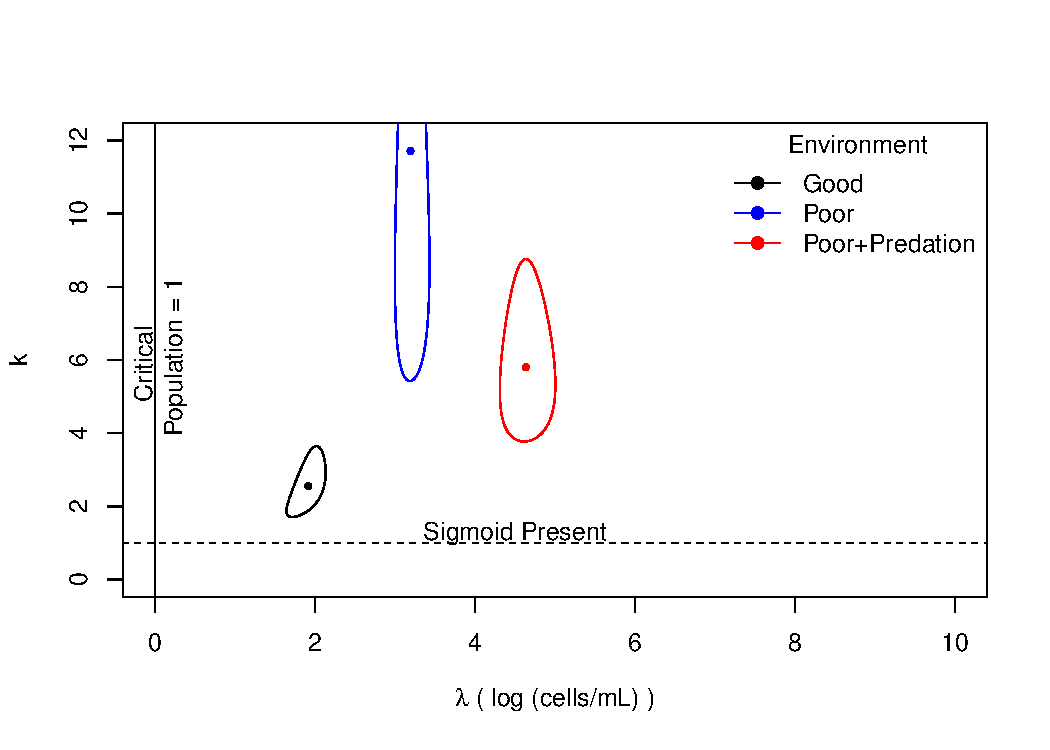
\includegraphics{MS_v1-fig1}
\end{center}
\caption{\textbf{Parameter estimates suggest Allee Effect present in all treatments.} The $k$ parameter is used to test the presence of an AE. Values greater than 1 indicate a sigmoidal relationship between density and probability of establishment. The shape parameter, $\lambda$, is the upper bound on the inflection point or critical density required to escape the AE. The point parameter estimates are presented with 95\% confidence intervals.  \textit{Include explanation of treatments?}
}
\end{figure}

\begin{figure}
\begin{center}
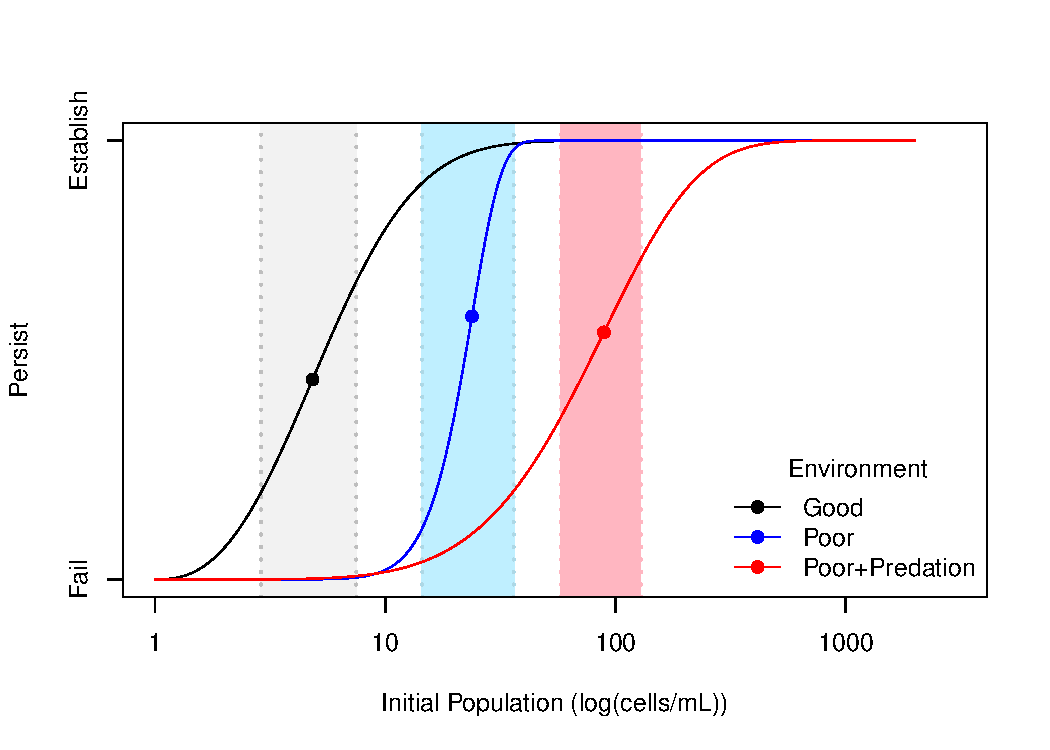
\includegraphics{MS_v1-fig2}
\end{center}
\caption{\textbf{Weibull curve based on estimated parameters.} Point is based on parameter point estimate, the shaded area is based on the 95\% confidence interval. The values are: X-X for the high resource (40mM glycerol), Y-Y low resource (20mM glycerol) and Z-Z low resource with predation (20mM glycerol plus 134 Cafeteria/mL)  
}
\end{figure}

\end{document}
